\documentclass[11pt,onside]{report}
\usepackage[a4paper]{geometry}
\usepackage[utf8]{inputenc}
\usepackage[english]{babel}
\usepackage{lipsum}
\usepackage{bm}
\usepackage{upgreek}
\usepackage{graphicx}
\usepackage[normalem]{ulem}

\usepackage{amsmath}
% mathtools for: Aboxed (put box on last equation in align envirenment)
\usepackage{microtype} %improves the spacing between words and letters

%% COLOR DEFINITIONS

\usepackage[svgnames]{xcolor} % Enabling mixing colors and color's call by 'svgnames'

\definecolor{MyColor1}{rgb}{0.2,0.4,0.6} %mix personal color
\newcommand{\textb}{\color{Black} \usefont{OT1}{lmss}{m}{n}}
\newcommand{\blue}{\color{MyColor1} \usefont{OT1}{lmss}{m}{n}}
\newcommand{\blueb}{\color{MyColor1} \usefont{OT1}{lmss}{b}{n}}
\newcommand{\red}{\color{LightCoral} \usefont{OT1}{lmss}{m}{n}}
\newcommand{\green}{\color{Turquoise} \usefont{OT1}{lmss}{m}{n}}

\DeclareMathOperator{\trace}{trace}
\DeclareMathOperator{\diag}{diag}

%% FONTS AND COLORS

%    SECTIONS

\usepackage{titlesec}
\usepackage{sectsty}
%%%%%%%%%%%%%%%%%%%%%%%%
%set section/subsections HEADINGS font and color
\sectionfont{\color{MyColor1}}  % sets colour of sections
\subsectionfont{\color{MyColor1}}  % sets colour of sections

%set section enumerator to arabic number (see footnotes markings alternatives)
\renewcommand\thesection{\arabic{section}.} %define sections numbering
\renewcommand\thesubsection{\thesection\arabic{subsection}} %subsec.num.

%define new section style
\newcommand{\mysection}{
\titleformat{\section} [runin] {\usefont{OT1}{lmss}{b}{n}\color{MyColor1}} 
{\thesection} {3pt} {} } 


%	CAPTIONS
\usepackage{caption}
\usepackage{subcaption}
%%%%%%%%%%%%%%%%%%%%%%%%
\captionsetup[figure]{labelfont={color=Turquoise}}


%		!!!EQUATION (ARRAY) --> USING ALIGN INSTEAD
%using amsmath package to redefine eq. numeration (1.1, 1.2, ...) 
\renewcommand{\theequation}{\thesection\arabic{equation}}



\makeatletter
\let\reftagform@=\tagform@
\def\tagform@#1{\maketag@@@{(\ignorespaces\textcolor{red}{#1}\unskip\@@italiccorr)}}
\renewcommand{\eqref}[1]{\textup{\reftagform@{\ref{#1}}}}
\makeatother
\usepackage{hyperref}
\hypersetup{colorlinks=true}

% For labeling top of page on every page but first one:
\usepackage{fancyhdr}

% PREPARE TITLE:
\title{\blue COMP 354 \\
\blueb Deliverable 1 \\ \blue Team I}

\author{
  Michael Marcelino \and
  Sobhan Mehrpour Kevishahi \and
  Hao Mei \and 
  Robert Michaud \and
  Elijah Mon \and
  Xavier Morin \and
  Chelsie Ng Man King}
  
\date{14-June-2021} % You can set the date automatically by replacing "date goes here" with "\today"

\renewcommand{\rmdefault}{phv} % Arial Font
\renewcommand{\sfdefault}{phv} % Arial Font

\pagestyle{fancy}
\fancyhead{}
\fancyhead[CO,CE]{{\small{{\bf{Deliverable 1}} - COMP 354 - Summer 2021 - Team I}}}
 


\begin{document}
\maketitle
\tableofcontents{}
\newpage
\section{Glossary}

% Glossary is arranged in alphabetical order.
\begin{itemize}
    
    \item \textbf{Back-End:} In the realm of software engineering, back-end often refers to the code that is responsible for the logic of a system, but which the user never directly interacts with through the user interface. \cite{sonmez_2017}
    
    \item \textbf{ETERNITY:} The name of our web-based calculator. 
    
    \item \textbf{Front-End:} In the realm of software engineering, front-end refers to the code that is responsible for the user interface and user experience. It is the part of the software that a user interacts with. \cite{naor_2021}
    
    \item \textbf{Full-Stack:} In the realm of software engineering, full-stack refers to both the front-end and back-end code and their integration with one another.

    \item \textbf{Function:} An assignment from an element of one set to exactly one element of the second set. \cite{function}. Alternatively, in this project it is also a shorthand for the eight transcendental functions that are part of ETERNITY.
    
    \item \textbf{Persona:} Personas define who you're designing your product for and are based on real user data. Personas create a common language for everyone designing the product and avoids the ambiguous term "users." \cite{personas}
    
    \item \textbf{Scientific Calculator:}  An electronic calculator that can handle trigonometric, exponential and often other advance functions. The output is generally showed in scientific notation. \cite{scientific}
    
    \item \textbf{Software:} A set of instructions and data that operates a computer and tells it what to do. \cite{software}  The term is an opposition to hardware which designate the tangible or physical parts of a computer. 
    
    \item \textbf{Standard Calculator:} A usually electronic device for performing mathematical calculations. \cite{calculator}
    
    \item \textbf{User:} Within the context of the ETERNITY project, a user is a person who will directly interact with the software.
    
    \item \textbf{User Experience:} Often referred to as UX, the user experience is how a user interacts with and experiences a product, system or service. It includes a person's perceptions of utility, ease of use, and efficiency. \cite{ux}
    
    \item \textbf{User Interface:} Often referred to as UI, the user interface is the space where interactions between humans and machines occur. \cite{ui}
    
\end{itemize}

\section{Collaboration Patterns And Tools}
\begin{description}
In order to maximize our team's productivity and efficiency, we decided to use a number of collaboration tools to streamline the creation of ETERNITY. Below you'll find the three main tools used to accomplish this.
\end{description}

% List of collaboration tools.
\begin{itemize}

    \item \textbf{Discord:} Discord is a voice, video, and text communication service \cite{discord}. We chose it for the following reasons:
    % Reasons:
    \begin{enumerate}
        \item \textbf{Familiarity:} All members of the group had previously used Discord, so everyone was already familiar with the interface and basic set of features. No extra time was needed to learn it.
        
        \item \textbf{Features:} Discord offers the ability to create different text channels which we have used to keep track of different types of information — including notes, meeting information, and discussions on the deliverables. 
        
        It also offers voice channels which we use for weekly meetings. These also offer the ability to share screens, which has helped get everyone on the same page when reviewing project requirements or asking about new technologies.
        
        \item \textbf{Portability:} Discord is available on a web browser, as a desktop program, and on mobile devices. This allows us to communicate in nearly all circumstances.
    \end{enumerate}
    
    \item \textbf{GitHub:} A platform where developers build, ship, and maintain their software \cite{github}. We chose it for the following reasons:
    
    \begin{enumerate}
        \item \textbf{Version Control:} GitHub builds off of Git, which is a version control system. By using GitHub we are adding version control to our work, allowing us to track positive and negative changes in the software and make changes accordingly. It also allows everyone’s code to use the most up-to-date version of other team member’s code. This helps avoid the needless redoing of previous work.
        
        \item \textbf{Project Management Features:} GitHub has a Kanban-like system integrated within, called GitHub Project. It allows collaborators to keep track of one another’s progress, and see the overall progress of the deliverables. It is also directly linked with GitHub's issue feature.
        
        \item \textbf{Wiki Features:} GitHub has a built-in wiki feature that allows collaborators to create wikis and glossaries for their projects. It's also a great place to keep documentation regarding the software. Since a glossary is already a requirement for the deliverables, this seemed like a great feature to use. It also allowed us to slowly create parts of the report as the project progressed, so the report only involves us porting the information we have from the Wiki to a \LaTeX{} report.
    \end{enumerate}
    
    \item \textbf{Google Documents:} An online word processor. We chose it for the following reasons:
    
    \begin{enumerate}
        \item \textbf{Collaborative Ability:} Google Documents allows multiple collaborators to work on a single document at the same time. This allows more cohesion and enables the work to break down a large task into smaller chunks and work through it that way.
        
        \item \textbf{Cloud Functionality:} All Google Documents reside on the cloud, so all members access the same document. This creates a single source of information for collaborators, allowing everyone to stay on the same page. Or to jot down ideas in a relatively unformatted way. While GitHub could be used instead, its focus on source code limits the flexibility of the types of notes taken — an issue not present in Google Documents.
    \end{enumerate}
\end{itemize}

\section{Role Assignment}
\begin{description}
For a team to work together effectively, there need to be some well-defined roles so everyone understands their responsibilities. That is why our team was quick to assign roles. These were based on both a person's preference and skills, so everyone could contribute in something they were comfortable and skilled at.
\end{description}
\begin{center}
\begin{tabular}{|l|l|}
    \hline
    \bf{Person} & \bf{Role(s)}  \\
    \hline
    Chelsie & Full-Stack \\
    \hline
    Elijah & Back-End \\
    \hline
    Hao & Communication, Organizer \\
    \hline
    Michael & Front-End, Major Presenter \\
    \hline
    Robert & Group Leader, Minor Presenter \\
    \hline
    Sobhan & Documentation, Wiki, Use Cases \\
    \hline
    Xavier & Documentation, \LaTeX{} \\
    \hline
\end{tabular}
\end{center}

\section{Function Mapping}
\begin{description}
To comply with the rules of the project, each team member was assigned one of the eight transcendental functions we are meant to implement. Seeing as there were only seven team members, we agreed not to do $\Gamma{}(x)$. \\ \\

Each person was given time to learn more about the various functions, and we all picked the functions during a single meeting. We went person to person and asked which function that person would like to implement, which resulted in the following function assignment:
\end{description}

\begin{center}
\begin{tabular}{|l|l|}
    \hline
    \bf{Person} & \bf{Function}  \\
    \hline
    Chelsie & $\sigma{}$ (Standard Deviation) \\
    \hline
    Elijah & $\sinh{x}$ \\
    \hline
    Hao & $ab^x$ \\
    \hline
    Michael & $x^y$ \\
    \hline
    Robert & $\arccos{x}$ \\
    \hline
    Sobhan & MAD (Mean Absolute Deviation) \\
    \hline
    Xavier & $\log{}_bx$ \\
    \hline
\end{tabular}
\end{center}

\section{Function Definitions}
\begin{description}
Here are the definitions and implementations of seven of the transcendental functions.
\end{description}

\subsection{$\sigma$ (Standard Deviation)}
\begin{description}
    Standard deviation is a measure of how spread out numbers are, and it is represented by the Greek letter sigma, $\sigma$. \\
    The formal definition is as follows:
\end{description}
\begin{equation}
    \sigma = \sqrt{\frac{\sum |x-\mu|^2}{N}}
\end{equation}
\begin{description}
Where $x$ is a data point, $\mu$ is the mean of the data set, and $N$ is the number of data points. \cite{standard_deviation}
\end{description}

\subsection{$\sinh{x}$}
\begin{description}
The hyperbolic sine function is similar to the trigonometric sine function, but is based on a hyperbola instead of a circle. \cite{sinh}
\end{description}
\begin{equation}
    \sinh{x} = \frac{e^x-e^{-x}}{2}
\end{equation}

\subsection{$ab^x$}
\begin{description}
This is the exponential function and includes the exponentiation operation, which is described in the next section. \\
Let $m$ be the exponentiation $b^x$, then
\end{description}
\begin{equation}
    ab^x = a\times m
\end{equation}

\subsection{$x^y$}
\begin{description}
The exponentiation operator has several definitions. The most common is when $y$ is an integer, in which case $x^y = x \times x \times ... \times x$ ($y$ times). If $y = 0$, then $x^y = 1$, and if $y < 0$, then $x^y = \frac{1}{x^{|y|}}$. \cite{exponents}\\ \\

Yet if $y$ is a real number, then it can often only be approximated using a Taylor series or other means of approximation. \\ \\

One important instance of $x^y$ is $e^y$ which is defined as $e^y = \lim_{n \to \infty} (1 + \frac{y}{n})^n$. \cite{e^x}
\end{description}

\subsection{$\arccos{x}$}
\begin{description}
$\arccos{x}$ is an inverse trigonometric function. It is the inverse function of $\cos{x}$ with a limited domain. \\ \\

If $y = \cos{x}$ then $x = \arccos{y}$, where $-1 \leq x \leq 1$ and $0 \leq y \leq \pi$. \cite{arccos}
\end{description}

\subsection{MAD (Mean Absolute Deviance)}
\begin{description}
Let $\mu$ be the average value in a data set of size $n$, and let $x_i$ be a value in this set. The mean absolute deviance is defined as \cite{mad}
\end{description}
\begin{equation}
    \frac{1}{n}\sum_{i=1}^{n}|x_i-\mu|
\end{equation}

\subsection{$\log_b(x)$}
\begin{description}
$\log_b(x)$ is defined as $\frac{\ln(x)}{\ln(b)}$, where $\ln(x)$ is the natural logarithm with base $e$ (though this identity holds for other bases as well). \cite{log}\\ \\

If $y = e^x$, then the natural logarithm is the inverse such that $x = \ln(y)$. \cite{ln}
\end{description}

\section{Interviews}
\subsection{Target Audience}
\begin{description}
Before beginning the interview, we realized we needed to have an idea of who would want to use the ETERNITY calculator. Obviously, a lot of people use calculators, but only a small subset of them would use the kinds of functions that ETERNITY would include. Therefore, we did some brainstorming during one of our group meetings and came up with the following target audience:
\end{description}
\begin{itemize}
    \item Students
    \item Statisticians
    \item Data Analysts
    \item Businessmen
    \item Accountants
    \item Engineers
    \item Professors
\end{itemize}
\begin{description}
These groups helped us decide who to interview, what kind of questions to ask, and eventually the personas themselves.
\end{description}

\subsection{Interview Format}
\begin{description}
Before creating the interview questions, we unanimously agreed to go for a semi-structured format of interview. This is because the majority of our team did not have experience interviewing people, so an open interview structure was not feasible at our skill level. A fully-structured interview was possible, but we were worried that a rigid structure would limit what we could learn from our interviewees. \\ \\

We then chose the funnel model of interviews, where we start off with general questions and become more specific as the interview progresses. We believe that this ease's the interviewee's mind into the topic, allowing them to think more critically about the topic so that we can gain more useful information.
\end{description}

\subsection{Interview Questions}
\begin{description}
We developed the interview questions by telling each member of our team to come up with five questions in the shared Google Document, for a total of thirty-five questions. We then filtered, refined, and structured the questions down to thirty, as seen below:
\end{description}
\begin{enumerate}
    \item What is your age?
    \item Which languages are you capable of speaking fluently?
    \item What is your current employment status? If you are employed, what do you do?
    \item What is the highest degree or level of education you have completed?
    \item How would you describe your technological literacy level?
    \begin{enumerate}
        \item Very Good
        \item Good
        \item Average
        \item Below Average
        \item Not Good
    \end{enumerate}
    \item How often do you use technology (computers, software, other hardware) on a daily basis?
    \begin{enumerate}
        \item Very often (more than twice a day)
        \item Often (twice a day)
        \item Once a day
        \item Less than once a day
        \item Once a week
    \end{enumerate}
    \item As a follow-up to my previous question, what software, if any, do you use on a day to day basis?
    \item In your work, do you like to use real tools or virtual network tools to complete your tasks through your computer? Handheld calculator vs. online calculator for example.
    \item Do you use calculators often? If so, in what setting and for what purpose?
    \item Are you familiar with transcendental functions? If so, which functions do you find yourself using most often than others?
    \item What is your level of proficiency regarding a calculator? (How many functions do you use or know how to use on a normal calculator, e.g. CASIO)
    \item If you find yourself using a calculator, what functions or types of calculations do you use/perform?
    \item Does the complexity or features offered by a calculator matter? Will it affect which type of calculator you choose to buy or use over another?
    \item As a follow-up to my previous question, does the appearance or size of the calculator matter to you? Explain.
    \item When using a calculator at work, or for personal use, is the degree of precision important? i.e. are you calculating sensitive data or not?
    \item If applicable, do you find yourself switching calculators throughout the day? Either at work or at home. If not, do you simply prefer to have a single calculator that offers every possible function needed?
    \item Are you open to the idea of trying alternative tools, or do you prefer to sticking to what you are already using? If not, please explain why.
    \item What best describes your willingness to try alternatives?
    \begin{enumerate}
        \item Curiosity
        \item Better performance/ precision/ job done better
        \item Didn’t like current tool
        \item Other (explain)
    \end{enumerate}
    \item Which alternative strikes you as the most practical:
    \begin{enumerate}
        \item a calculator app on your phone,
        \item a web app accessible from any device with Internet access,
        \item a physical calculator
        \item a desktop application, such as the default Windows calculator?
    \end{enumerate}
    \item Have you ever used an online calculator?
    \item If you have used an online calculator before, what were some of the difficulties you experienced with it? If not, would you use an online calculator?
    \item As a follow-up to my previous question: If so what features or functions would you be interested in using/having in an online calculator? If not, why not?
    \item Would customizability be a factor in choosing whether to use an online calculator over an alternative, yes or no?
    \item Can you name 3 of your favorite calculator applications or alternatively, 3 of your favorite handheld calculator brands?
    \item What aspect of these applications or calculators appeals to you the most?
    \item Have you used your operating system’s default calculator? If so, what did you like and dislike about it?
    \item When using a calculator, does the appearance of the math expression matter to you? (x\^{}y vs $x^y$).
    \item How often do you use trigonometric functions? And when using them, do you prefer to use radians or degrees? Do you like having the ability to switch between them?
    \item Which functions that are generally not on a calculator, would you like to see added?
    \item That’s all for the interview. Do you have any questions for myself or things you’d like to add? Are there things that you’d like to discuss regarding either online calculators, calculators in general, or even different online tools/software?
\end{enumerate}

\section{Transcripts}
\begin{description}
    Here you'll find the transcripts of the seven interviews.
\end{description}
\subsection{Interview 1}
\begin{enumerate}
    \item What is your age? \\
    \blue 22. \textb
    
    \item Which languages are you capable of speaking fluently? \\
    \blue English, French, and Chinese. \textb \\
    Mandarin? \\
    \blue Yes. \textb
    
    \item What is your current employment status? If you are employed, what do you do? \\
    \blue I’m going to start a new part-time job next week. \textb \\
    And what is that? \\
    \blue I will be a marketing specialist. \textb \\
    Okay, for which company, if you don’t mind? \\
    \blue For Unilever Canada under the shopper-marketing department. \textb \\ 
    You mentioned that you will be starting your internship soon. Have you had another internship
recently? \\
    \blue Yes, I was a customer development intern for Unilever Canada during the winter semester. \textb
    
    \item What is the highest degree or level of education you have completed? \\
    \blue Cegep. But, right now I’m pursuing my bachelor degree of Commerce, specializing in marketing. I
will graduate in August. \textb
    
    \item How would you describe your technological literacy level?
    \begin{enumerate}
        \item Very Good
        \item Good
        \item Average
        \item Below Average
        \item Not Good
    \end{enumerate} \\
    \blue I would say average \textb \\
    Could you elaborate? \\
    \blue I can function using day-to-day technology, laptop, ipad, etc… But I wouldn’t be using anything
    that takes some research to be able to learn the technology. \textb \\
    Alright, so you wouldn’t be doing any troubleshooting or anything like that, right? \\
    \blue Exactly. \textb
    
    \item How often do you use technology (computers, software, other hardware) on a daily basis?
    \begin{enumerate}
        \item Very often (more than twice a day)
        \item Often (twice a day)
        \item Once a day
        \item Less than once a day
        \item Once a week
    \end{enumerate} \\
    \blue Very often, more than twice a day for sure. \textb
    
    \item As a follow-up to my previous question, what software, if any, do you use on a day to day basis? \\
    \blue I use Android. \textb \\
    Okay, so do you use a browser? \\
    \blue Yes, I use Google Chrome. \textb \\
    Do you use any other software, like Microsoft Word, Powerpoint, etc. \\
    \blue Yes, I use Microsoft Office, so, like Power BI, Word, Excel, PowerPoint, etc. \textb \\
    Okay, on Power BI and Excel, do you do a lot of calculation? \\
    \blue Yeah, I do a lot of analysis on Excel, and sometimes on Power BI. \textb
    
    \item In your work, do you like to use real tools or virtual network tools to complete your tasks through your computer? Handheld calculator vs. online calculator for example. \\
    \blue I like to use virtual tools to do my daily work. I have a work laptop so we usually do everything
on the computer. \textb

    \item Do you use calculators often? If so, in what setting and for what purpose? \\
    \blue Yes, I’ll use one multiple times a week. In the setting of my work, for instance, especially during
my previous internship, it was a lot of analysis about prices, numbers, sales volume, percentage,
etc. So to double check everything that was automatic on Excel, I would just use the online calculator to double check my numbers. \textb \\
    Wait, so you used an online calculator? \\
    \blue I type “calculator” on my laptop, and an app comes out. \textb \\
    Oh, so the Microsoft Calculator? \\
    \blue Yeah, the one that comes with the laptop. \textb
    
    \item Are you familiar with transcendental functions? If so, which functions do you find yourself using most often than others? \\
    \blue I am not. \textb
    
    \item What is your level of proficiency regarding a calculator? (How many functions do you use or know how to use on a normal calculator, e.g. CASIO) \\
    \blue I really only use the basic functions. \textb \\
    So you use sum, minus, division, etc. But do you use power, sqrt, etc? \\
    \blue For work, no. But I did have to use it for school, yeah. \textb
    
    \item If you find yourself using a calculator, what functions or types of calculations do you use/perform? \\
    \blue So, usually, for work I only use basic functions such as addition, division, multiplication and
subtraction. \textb

    \item Does the complexity or features offered by a calculator matter? Will it affect which type of calculator you choose to buy or use over another? \\
    \blue Honestly, I don’t mind but I really only need a simple calculator. \textb
    
    \item As a follow-up to my previous question, does the appearance or size of the calculator matter to you? Explain. \\
    \blue You mean online? \textb \\
    Just in general, it doesn't matter. \\
    \blue If it’s physical, I prefer my calculator to be pink. If it’s online, then no, it doesn’t matter. If it’s
simple to use, I am OK. \textb

    \item When using a calculator at work, or for personal use, is the degree of precision important? i.e. are you calculating sensitive data or not? \\
    \blue Oh, no it doesn’t really matter. Most of the time, I’m dealing with dollars, so as long as there is
two decimal precision for the cents, I’m OK. \textb

    \item If applicable, do you find yourself switching calculators throughout the day? Either at work or at home. If not, do you simply prefer to have a single calculator that offers every possible function needed? \\
    \blue I don’t. I would prefer to have a single calculator that offers everything I need. \textb
    
    \item Are you open to the idea of trying alternative tools, or do you prefer to sticking to what you are already using? If not, please explain why. \\
    \blue Could you elaborate on “alternative tools”? \textb \\
    So, for example you’re already using a word processor that you’re used to. Would you be open to trying another one? Or in our case, you’re used to the Microsoft calculator, but would you be open to trying a different one. \\
    \blue Yes. \textb
    
    \item What best describes your willingness to try alternatives?
    \begin{enumerate}
        \item Curiosity
        \item Better performance/ precision/ job done better
        \item Didn’t like current tool
        \item Other (explain)
    \end{enumerate} \\
    \blue     If it has better performance, is more precise or adds value to my day-to-day work, then I’d be open to trying it out.\textb
    
    \item Which alternative strikes you as the most practical:
    \begin{enumerate}
        \item a calculator app on your phone,
        \item a web app accessible from any device with Internet access,
        \item a physical calculator
        \item a desktop application, such as the default Windows calculator?
    \end{enumerate} \\
    \blue A Desktop application. If it’s for work, sometimes, I won’t have my phone next to me. But, for day-to-day tasks, like if there’s a big promotion when I’m grocery shopping, then I like to use my phone since I don’t have my laptop and it’s more convenient. \textb
    
    \item Have you ever used an online calculator? \\
    \blue Yes. \textb
    
    \item If you have used an online calculator before, what were some of the difficulties you experienced with it? If not, would you use an online calculator? \\
    \blue There wasn’t much of a difficulty. It was more about the fact that I had to type “calculator” on Google and had to click a link. So right now, I’d rather just use an app on my laptop because it’s easier. \textb
    
    \item As a follow-up to my previous question: If so what features or functions would you be interested in using/having in an online calculator? If not, why not? \\
    \blue Just the basic functions, like I mentioned before. \textb 
    
    \item Would customizability be a factor in choosing whether to use an online calculator over an alternative, yes or no? \\
    \blue Customizability… so like, the appearance of the calculator? \textb \\
    Yes, so for example, a light or dark theme. Or, like you said, you like to have a pink calculator, so there could be a pink theme for an online calculator. \\
    \blue ...Yes, it [opinion] would change  a lot. If I could choose the appearance of the online calculator, I’d choose something like a Sailor Moon theme, and for sure I would use that over any other calculator... \textb

    
    \item Can you name 3 of your favorite calculator applications or alternatively, 3 of your favorite handheld calculator brands? \\
    \blue I like Casio because I’ve used the brand through highschool, cegep and university. And they also make a pink version, which I have. \textb \\
    And you mentioned that you like the Windows Calculator because it’s easy to uset? \\
    \blue Yeah, I like it because it’s easy to use. I just have to open the search bar on my laptop and type “ca-” and it will show up. \textb
    
    \item \sout{What aspect of these applications or calculators appeals to you the most?}
    
    \item \sout{Have you used your operating system’s default calculator? If so, what did you like and dislike about it?} Speaking of the Windows Calculator, is there anything that you dislike, or like about it? \\
    \blue Like about it… nothing. Dislikes, I would prefer to be able to customize the look of the calculator, I think that would be very cool. \textb 
    
    \item When using a calculator, does the appearance of the math expression matter to you? (x\^{}y vs $x^y$). \\
    \blue Yeah, so for example I prefer to see the actual fraction, with the line and both numbers on top and at the bottom. I used both types and I much prefer to be able to see it. And for the exponents, I also prefer the option where you see it on top [not \^{}]. \textb
    
    \item How often do you use trigonometric functions? And when using them, do you prefer to use radians or degrees? Do you like having the ability to switch between them? \\
    \blue Not anymore, I used to use it for class but not anymore. \textb 
    
    \item Which functions that are generally not on a calculator, would you like to see added? \\
    \blue I’m good. \textb
    
    \item That’s all for the interview. Do you have any questions for myself or things you’d like to add? Are there things that you’d like to discuss regarding either online calculators, calculators in general, or even different online tools/software? \\
    \blue Are you guys building a calculator? \textb \\
    Yes, we’re making an online calculator. \\
    \blue Wow, that’s cool. Will we be able to use it, and will we be able to customize it? \textb \\
    Yeah, for sure. For customizability, since there is demand for it,  I think that’s something we want to implement. \\
    \blue That’d be great. It would be fun to see different colours and themes.\textb
\end{enumerate}

\subsection{Interview 2}
\begin{enumerate}
    \item What is your age? \\
    \blue 45. \textb
    
    \item Which languages are you capable of speaking fluently? \\
    \blue English and Chinese (Mandarin) \textb
    
    \item What is your current employment status? If you are employed, what do you do? \\
    \blue Permanent Employee, I am a cost estimator.  \textb
    
    \item What is the highest degree or level of education you have completed? \\
    \blue Master in Engineering. \textb
    
    \item How would you describe your technological literacy level?
    \begin{enumerate}
        \item Very Good
        \item \blue Good \textb
        \item Average
        \item Below Average
        \item Not Good
    \end{enumerate}
    
    \item How often do you use technology (computers, software, other hardware) on a daily basis?
    \begin{enumerate}
        \item \blue Very often (more than twice a day) \textb
        \item Often (twice a day)
        \item Once a day
        \item Less than once a day
        \item Once a week
    \end{enumerate}
    
    \item As a follow-up to my previous question, what software, if any, do you use on a day to day basis? \\
    \blue Microsoft Excel, Words, PowerPoint; Prism; InEight; AutoCAD; \textb
    
    \item In your work, do you like to use real tools or virtual network tools to complete your tasks through your computer? Handheld calculator vs. online calculator for example. \\
    \blue Like to use online tools; \textb

    \item Do you use calculators often? If so, in what setting and for what purpose? \\
    \blue No, don’t use it very often. \textb
    
    \item Are you familiar with transcendental functions? If so, which functions do you find yourself using most often than others? \\
    \blue No. \textb
    
    \item What is your level of proficiency regarding a calculator? (How many functions do you use or know how to use on a normal calculator, e.g. CASIO) \\
    \blue Basic functions.  \textb
    
    \item If you find yourself using a calculator, what functions or types of calculations do you use/perform? \\
    \blue  “+, -, ×,÷”. \textb

    \item Does the complexity or features offered by a calculator matter? Will it affect which type of calculator you choose to buy or use over another? \\
    \blue Doesn’t matter. I don’t use the real calculator most of time. \textb
    
    \item As a follow-up to my previous question, does the appearance or size of the calculator matter to you? Explain. \\
    \blue No. \textb

    \item When using a calculator at work, or for personal use, is the degree of precision important? i.e. are you calculating sensitive data or not? \\
    \blue Yes, the figure accurate to four decimal places would be ok. \textb

    \item If applicable, do you find yourself switching calculators throughout the day? Either at work or at home. If not, do you simply prefer to have a single calculator that offers every possible function needed? \\
    \blue The software I use has function to do calculation.  \textb
    
    \item Are you open to the idea of trying alternative tools, or do you prefer to sticking to what you are already using? If not, please explain why. \\
    \blue yes. I open to alternative tool if it is more simple and easy to use. \textb
    
    \item What best describes your willingness to try alternatives?
    \begin{enumerate}
        \item Curiosity
        \item \blue Better performance/ precision/ job done better \textb
        \item Didn’t like current tool
        \item Other (explain)
    \end{enumerate}
    
    \item Which alternative strikes you as the most practical:
    \begin{enumerate}
        \item a calculator app on your phone,
        \item a web app accessible from any device with Internet access, 
        \item a physical calculator
        \item \blue a desktop application, such as the default Windows calculator? \textb
    \end{enumerate}
    
    \item Have you ever used an online calculator? \\
    \blue Yes. \textb
    
    \item If you have used an online calculator before, what were some of the difficulties you experienced with it? If not, would you use an online calculator? \\
    \blue Yes, I like to use online calculator. \textb
    
    \item As a follow-up to my previous question: If so what features or functions would you be interested in using/having in an online calculator? If not, why not? \\
    \blue Convenience to use, easy to reach. \textb 
    
    \item Would customizability be a factor in choosing whether to use an online calculator over an alternative, yes or no? \\
    \blue Yes, but it is not necessary for me \textb

    
    \item Can you name 3 of your favorite calculator applications or alternatively, 3 of your favorite handheld calculator brands? \\
    \blue Scientific Calculator (just use a normal online calculator) \textb
    
    \item What aspect of these applications or calculators appeals to you the most? \\
    \blue Convenient, fast, and accurate calculation \textb
    
    \item Have you used your operating system’s default calculator? If so, what did you like and dislike about it? \\
    \blue Yes.  I like that it is easy to reach, dislike: it is not easy to use, except to have a touchable screen. \textb 
    
    \item When using a calculator, does the appearance of the math expression matter to you? (x\^{}y vs $x^y$). \\
    \blue Yes, standard expression would be better. \textb
    
    \item How often do you use trigonometric functions? And when using them, do you prefer to use radians or degrees? Do you like having the ability to switch between them? \\
    \blue Sometimes. I prefer to use degree. If have the ability to switch between radians and degrees would be great. \textb 
    
    \item Which functions that are generally not on a calculator, would you like to see added? \\
    \blue No. For me, ordinary calculators have met my work needs. \textb
    
    \item That’s all for the interview. Do you have any questions for myself or things you’d like to add? Are there things that you’d like to discuss regarding either online calculators, calculators in general, or even different online tools/software? \\
    \blue No. But I wish you success in creating your calculator! \textb
\end{enumerate}

\subsection{Interview 3}
\begin{enumerate}
    \item What is your age? \\
    \blue 21. \textb
    
    \item Which languages are you capable of speaking fluently? \\
    \blue Mauritian Creole, French and English. \textb
    
    \item What is your current employment status? If you are employed, what do you do? \\
    \blue I am an undergraduate student and this Summer is my last semester.  \textb \\
    And what is your field of study? \\
    \blue Computer Science \textb
    
    \item What is the highest degree or level of education you have completed? \\
    \blue High School. \textb
    
    \item How would you describe your technological literacy level?
    \begin{enumerate}
        \item Very Good
        \item Good
        \item Average
        \item Below Average
        \item Not Good
    \end{enumerate} \\
    \blue Very good. \textb
    
    \item How often do you use technology (computers, software, other hardware) on a daily basis?
    \begin{enumerate}
        \item Very often (more than twice a day)
        \item Often (twice a day)
        \item Once a day
        \item Less than once a day
        \item Once a week
    \end{enumerate} \\
    \blue Very often. Actually, I am a software developer so I work with technology every day. \textb
    
    \item As a follow-up to my previous question, what software, if any, do you use on a day to day basis? \\
    \blue Phone, my laptop, social media. \textb \\
    Which phone, laptop, social media? \\
    \blue Oneplus 6T, Huawei matebook x pro, Facebook, Instagram, YouTube.  \textb
    
    \item In your work, do you like to use real tools or virtual network tools to complete your tasks through your computer? Handheld calculator vs. online calculator for example. \\
    \blue Whatever is the most convenient. In an exam, I will use my real calculator but in everyday life, I won’t bother looking for my calculator, I will just perform calculations on my phone. \textb

    \item Do you use calculators often? If so, in what setting and for what purpose? \\
    \blue Yes I use it for school and in my everyday life, such as calculating the cost of my groceries or any other payments. \textb
    
    \item Are you familiar with transcendental functions? If so, which functions do you find yourself using most often than others? \\
    \blue Yes, I most often used trigonometric functions in my high school years. These functions were only used for academic purposes and not for my personal life. \textb \\
    How about during university? \\
    \blue That’s what I meant, high school, uni, academic purposes, same thing. \textb
    
    \item What is your level of proficiency regarding a calculator? (How many functions do you use or know how to use on a normal calculator, e.g. CASIO) \\
    \blue I know how to use everything man.  \textb
    
    \item If you find yourself using a calculator, what functions or types of calculations do you use/perform? \\
    \blue The basic things. Simple addition, subtraction, division, multiplication and functions that my math classes use. Eg, trigonometric functions. \textb

    \item Does the complexity or features offered by a calculator matter? Will it affect which type of calculator you choose to buy or use over another? \\
    \blue Yes the more features the better so that I am not limited. Appearance also matters. \textb
    
    \item As a follow-up to my previous question, does the appearance or size of the calculator matter to you? Explain. \\
    \blue As I said above, yes. I like to use something good looking. \textb

    \item When using a calculator at work, or for personal use, is the degree of precision important? i.e. are you calculating sensitive data or not? \\
    \blue No if I was using it for academic purposes it would matter but at work or in my personal life it is not an issue. \textb

    \item If applicable, do you find yourself switching calculators throughout the day? Either at work or at home. If not, do you simply prefer to have a single calculator that offers every possible function needed? \\
    \blue Single calculator.  \textb
    
    \item Are you open to the idea of trying alternative tools, or do you prefer to sticking to what you are already using? If not, please explain why. \\
    \blue I prefer sticking to what I already have. I have no problem with my current calculator so I will not bother changing. \textb \\
    
    \item What best describes your willingness to try alternatives?
    \begin{enumerate}
        \item Curiosity
        \item \blue Better performance/ precision/ job done better \textb
        \item Didn’t like current tool
        \item Other (explain)
    \end{enumerate}
    
    \item Which alternative strikes you as the most practical:
    \begin{enumerate}
        \item a calculator app on your phone,
        \item \blue a web app accessible from any device with Internet access, \textb
        \item a physical calculator
        \item a desktop application, such as the default Windows calculator?
    \end{enumerate} \\
    \blue It would also be nice if the webapp is responsive for my phone and available offline. \textb
    
    \item Have you ever used an online calculator? \\
    \blue Yes. \textb
    
    \item If you have used an online calculator before, what were some of the difficulties you experienced with it? If not, would you use an online calculator? \\
    \blue The user interface and its use were not intuitive. E.g. WolframAlpha does provide symbols to write functions. \textb
    
    \item As a follow-up to my previous question: If so what features or functions would you be interested in using/having in an online calculator? If not, why not? \\
    \blue I prefer a scientific calculator. Every standard function you can find in a Casio calculator. More is better. Responsiveness of the online calculator is a must.  \textb 
    
    \item Would customizability be a factor in choosing whether to use an online calculator over an alternative, yes or no? \\
    \blue No. I prefer a simple calculator. \textb

    
    \item Can you name 3 of your favorite calculator applications or alternatively, 3 of your favorite handheld calculator brands? \\
    \blue I have only one favourite. Symbolab is the best so far. \textb
    
    \item What aspect of these applications or calculators appeals to you the most? \\
    \blue It’s user friendly. They have extensive functions available such as matrix calculations. The symbols and format of the equations are ready to be formatted by just clicking on them. \textb
    
    \item Have you used your operating system’s default calculator? If so, what did you like and dislike about it? \\
    \blue Yes. What I like about it is that it does what I want it to do. An improvement would be to have scientific functions as well and not only basic operations. \textb 
    
    \item When using a calculator, does the appearance of the math expression matter to you? (x\^{}y vs $x^y$). \\
    \blue It is a plus to display math expression like this $x^y$ but it does not bother me. \textb
    
    \item How often do you use trigonometric functions? And when using them, do you prefer to use radians or degrees? Do you like having the ability to switch between them? \\
    \blue Degrees and yes. \textb 
    
    \item Which functions that are generally not on a calculator, would you like to see added? \\
    \blue Mean, standard deviation, matrices. \textb
    
    \item That’s all for the interview. Do you have any questions for myself or things you’d like to add? Are there things that you’d like to discuss regarding either online calculators, calculators in general, or even different online tools/software? \\
    \blue No thank you. I am tired. I just got vaccinated. \textb
\end{enumerate}

\subsection{Interview 4}
\begin{enumerate}
    \item What is your age? \\
    \blue 20. \textb
    
    \item Which languages are you capable of speaking fluently? \\
    \blue I can speak English and Persian fluently. \textb
    
    \item What is your current employment status? If you are employed, what do you do? \\
    \blue Freelance. I work as a content creator and specialist.  \textb
    
    \item What is the highest degree or level of education you have completed? \\
    \blue I have completed secondary school and am currently in university. \textb \\
    And what are you studying in university? \\
    \blue Biology. \textb
    
    \item How would you describe your technological literacy level?
    \begin{enumerate}
        \item Very Good
        \item Good
        \item Average
        \item Below Average
        \item Not Good
    \end{enumerate} \\
    \blue Very good but not excellent. On a scale of 1 to 10, a 7 or 8. \textb
    
    \item How often do you use technology (computers, software, other hardware) on a daily basis?
    \begin{enumerate}
        \item Very often (more than twice a day)
        \item Often (twice a day)
        \item Once a day
        \item Less than once a day
        \item Once a week
    \end{enumerate} \\
    \blue Very often. \textb
    
    \item As a follow-up to my previous question, what software, if any, do you use on a day to day basis? \\
    \blue So I use Google Chrome, I use Notion, and Adobe Photoshop. \textb
    
    \item In your work, do you like to use real tools or virtual network tools to complete your tasks through your computer? Handheld calculator vs. online calculator for example. \\
    \blue Handheld calculator if I had to use a calculator. Since I use photo editing software for work, it’s virtual. \textb

    \item Do you use calculators often? If so, in what setting and for what purpose? \\
    \blue Yes. I use them for my education and just to study and for exams. \textb
    
    \item Are you familiar with transcendental functions? If so, which functions do you find yourself using most often than others? \\
    \blue I have heard of them. I believe I have dealt with them. [pause to think about it] Yes, I am aware of them and am familiar with them. Yes, I’d say I use them often. At least half of the time. \textb
    
    \item What is your level of proficiency regarding a calculator? (How many functions do you use or know how to use on a normal calculator, e.g. CASIO) \\
    \blue Just for basic things, like logarithms and trigonometric functions and basic division and multiplication and those basic functions.  \textb
    
    \item If you find yourself using a calculator, what functions or types of calculations do you use/perform? \\
    \blue I kind of answered that with my previous answer. So a little bit of everything. \textb

    \item Does the complexity or features offered by a calculator matter? Will it affect which type of calculator you choose to buy or use over another? \\
    \blue Yes. I have a TI Inspired CX calculator and I have a Casio calculator, but I always opt for the TI inspired unless it’s basic addition or multiplication. \textb
    
    \item As a follow-up to my previous question, does the appearance or size of the calculator matter to you? Explain. \\
    \blue To some extent. Shouldn’t be too large that you can’t carry it around or hold it in your hand. But shouldn’t be so small that you make mistakes when pressing buttons. But I don’t care about the colour or appearance. Just has to be easy to use. \textb

    \item When using a calculator at work, or for personal use, is the degree of precision important? i.e. are you calculating sensitive data or not? \\
    \blue In day to day, no. But for university there’s rigorous calculations so high degree is best. At least 3 decimal points. \textb

    \item If applicable, do you find yourself switching calculators throughout the day? Either at work or at home. If not, do you simply prefer to have a single calculator that offers every possible function needed? \\
    \blue Yes. \textb
    
    \item Are you open to the idea of trying alternative tools, or do you prefer to sticking to what you are already using? If not, please explain why. \\
    \blue If the alternate is much better, then I’d gladly switch. If it offers the same things as the tools I’m already using and it’s not really different, then I’ll continue using the tools I’m familiar with. \textb \\
    
    \item What best describes your willingness to try alternatives?
    \begin{enumerate}
        \item Curiosity
        \item Better performance/ precision/ job done better
        \item Didn’t like current tool
        \item Other (explain)
    \end{enumerate} \\
    \blue Curiosity. \textb
    
    \item Which alternative strikes you as the most practical:
    \begin{enumerate}
        \item a calculator app on your phone,
        \item a web app accessible from any device with Internet access,
        \item a physical calculator
        \item a desktop application, such as the default Windows calculator?
    \end{enumerate} \\
    \blue Can I choose two of them? \textb \\
    Sure thing. \\
    \blue One on my phone and a physical one. \textb
    
    \item Have you ever used an online calculator? \\
    \blue Yes. \textb
    
    \item If you have used an online calculator before, what were some of the difficulties you experienced with it? If not, would you use an online calculator? \\
    \blue Great question. Some online calculators say they perform a difficult task, but when the difficulty increases they break down and stop working. \textb
    
    \item As a follow-up to my previous question: If so what features or functions would you be interested in using/having in an online calculator? If not, why not? \\
    \blue It has to have a UX design and interface so it would be easy to use. I could see the solution easily and input the question or function easily. The placement of the functions should also be logical, since I sometimes spend 2 minutes searching for it.  \textb 
    
    \item Would customizability be a factor in choosing whether to use an online calculator over an alternative, yes or no? \\
    \blue Yes. \textb

    
    \item Can you name 3 of your favorite calculator applications or alternatively, 3 of your favorite handheld calculator brands? \\
    \blue TI Inspire CX, SymboLab, and I also use graphic calculators on my phone like Desmos and 3D Calculator. \textb
    
    \item What aspect of these applications or calculators appeals to you the most? \\
    \blue First of all speed. Symbolab is really quick when inputting the problem and getting the results. Accuracy which is what I like about Symbolab and TI Inspire. It just being easy to use, and can input things quickly. \textb
    
    \item Have you used your operating system’s default calculator? If so, what did you like and dislike about it? \\
    \blue Only if it’s very very very basic multiplication division. It doesn’t offer anything other than the basic calculations.  \textb \\
    And what operating systema are you using? \\
    \blue Mac OS \textb
    
    \item When using a calculator, does the appearance of the math expression matter to you? (x\^{}y vs $x^y$). \\
    \blue It would be best if it’s a superscript. Especially if it’s a long expression, since I’ll be more likely to make a mistake reading it otherwise. \textb
    
    \item How often do you use trigonometric functions? \\ 
    \blue Whenever I’m studying for math, which is several times a week.  \textb  \\
    And when using them, do you prefer to use radians or degrees? \\
    \blue Radians, unless vectors are involved. \textb \\
    Do you like having the ability to switch between them? \\
    \blue Yes \textb
    
    
    \item Which functions that are generally not on a calculator, would you like to see added? \\
    \blue Great question. Multivariable functions, whether in terms of graphing or finding the limits of. That’s pretty much it. Composite transcendental functions as well. \textb \\
    Could you elaborate on what you mean by composite transcendental functions? \\
    \blue Some calculators won’t really let you do e\^{}(x\^{}something). \textb
    
    \item That’s all for the interview. Do you have any questions for myself or things you’d like to add? Are there things that you’d like to discuss regarding either online calculators, calculators in general, or even different online tools/software? \\
    \blue Just pretty much what I said. Has to look good and be easy to use. And it’s best the symbols don’t look messed up or weird so you wouldn’t misunderstand or overlook them. \textb
\end{enumerate}
\subsection{Interview 5}
\begin{enumerate}
    \item What is your age? \\
    \blue I’m 38 year old. \textb
    
    \item Which languages are you capable of speaking fluently? \\
    \blue English is my first language and I am fluent in French, since I studied at the University of Montreal. \textb
    
    \item What is your current employment status? If you are employed, what do you do? \\
    \blue I work at IQVIA in the West of Montreal. I am employed as a statistician.   \textb
    
    \item What is the highest degree or level of education you have completed? \\
    \blue PhD in bio-statistics at University of Montreal. \textb \\
   
    
    \item How would you describe your technological literacy level?
    \begin{enumerate}
        \item Very Good
        \item Good
        \item Average
        \item Below Average
        \item Not Good
    \end{enumerate} \\
    \blue Very good\textb
    
    \item How often do you use technology (computers, software, other hardware) on a daily basis?
    \begin{enumerate}
        \item Very often (more than twice a day)
        \item Often (twice a day)
        \item Once a day
        \item Less than once a day
        \item Once a week
    \end{enumerate} \\
    \blue Very often. \textb
    
    \item As a follow-up to my previous question, what software, if any, do you use on a day to day basis? \\
    \blue I mainly deal with databases, SQL, Stata, VB and python. \textb
    
    \item In your work, do you like to use real tools or virtual network tools to complete your tasks through your computer? Handheld calculator vs. online calculator for example. \\
    \blue Most of our tools are partially virtual since the information is shared via a network, but my daily calculations, depending on the scale, are performed on my computer.
 \textb

    \item Do you use calculators often? If so, in what setting and for what purpose? \\
    \blue Less and less…  \textb
    
    \item Are you familiar with transcendental functions? If so, which functions do you find yourself using most often than others? \\
    \blue I am in fact familiar with those. I would say the logarithm. \textb
    
    \item What is your level of proficiency regarding a calculator? (How many functions do you use or know how to use on a normal calculator, e.g. CASIO) \\
    \blue Good question. I think I know how to use most of them.   \textb
    
    \item If you find yourself using a calculator, what functions or types of calculations do you use/perform? \\
    \blue The basics, plus, minus, multiplication, division, sin, cos, log, square root. \textb

    \item Does the complexity or features offered by a calculator matter? Will it affect which type of calculator you choose to buy or use over another? \\
    \blue It has to have more than the four basic operations.  Like you asked earlier, a Casio is perfect. \textb
    
    \item As a follow-up to my previous question, does the appearance or size of the calculator matter to you? Explain. \\
    \blue Not really, they all kind of look the same anyway. \textb

    \item When using a calculator at work, or for personal use, is the degree of precision important? i.e. are you calculating sensitive data or not? \\
    \blue I don’t think it ever causes me any problem. \textb

    \item If applicable, do you find yourself switching calculators throughout the day? Either at work or at home. If not, do you simply prefer to have a single calculator that offers every possible function needed? \\
    \blue I have a calculator at home and one at my desk, the rest of the time I would use my phone. \textb
    
    \item Are you open to the idea of trying alternative tools, or do you prefer to sticking to what you are already using? If not, please explain why. \\
    \blue I would be open minded, impress me.
 \textb \\
    
    \item What best describes your willingness to try alternatives?
    \begin{enumerate}
        \item Curiosity
        \item Better performance/ precision/ job done better
        \item Didn’t like current tool
        \item Other (explain)
    \end{enumerate} \\
    \blue Curiosity. \textb
    
    \item Which alternative strikes you as the most practical:
    \begin{enumerate}
        \item a calculator app on your phone,
        \item a web app accessible from any device with Internet access,
        \item a physical calculator
        \item a desktop application, such as the default Windows calculator?
    \end{enumerate} \\
    \blue A calculator app on your phone,  \textb 
    
    
    \item Have you ever used an online calculator? \\
    \blue I used Wolfram Alpha, but it's way more than a calculator. You can ask for any type integral for example. I think it can even tell you the weather.  \textb
    
    \item If you have used an online calculator before, what were some of the difficulties you experienced with it? If not, would you use an online calculator? \\
    \blue For Wolfram, much of the advanced stuff costs money, this generally bothers me. \textb
    
    
    \item Would customizability be a factor in choosing whether to use an online calculator over an alternative, yes or no? \\
    \blue Not really, maybe having a dark mode.
 \textb

    
    \item Can you name 3 of your favorite calculator applications or alternatively, 3 of your favorite handheld calculator brands? \\
    \blue Wolfram Alpha, Casio and Python :) \textb
    
    \item What aspect of these applications or calculators appeals to you the most? \\
    \blue Wolfram can pretty much solve anything, Casio is portable and straight to the point, Python you can do anything. \textb
    
    \item Have you used your operating system’s default calculator? If so, what did you like and dislike about it? \\
    \blue Yes for sure, for those kinds of calculations I always prefer to use the handheld one, that is why I always keep one at my desk.
  \textb \\
   
    
    \item When using a calculator, does the appearance of the math expression matter to you? (x\^{}y vs $x^y$). \\
    \blue Not really, I am used to different notations. However some are more elegant. \textb
    
    \item How often do you use trigonometric functions? \\ 
    \blue Not that often, but I am definitely on the radian team, it is so much more elegant, sorry to our Babylonian friends. Yes it could be convenient, why not.  \textb  \\
    
    
    
    \item Which functions that are generally not on a calculator, would you like to see added? \\
    \blue This is very difficult, maybe some constants could be added, like the gravity constant or the speed of light for our fellow engineer. 
 \textb \\
   
    
    \item That’s all for the interview. Do you have any questions for myself or things you’d like to add? Are there things that you’d like to discuss regarding either online calculators, calculators in general, or even different online tools/software? \\
    \blue I can’t wait to see your calculator, good luck.
 \textb
\end{enumerate}

\subsection{Interview 6}
\begin{enumerate}
    \item What is your age? \\
    \blue You know my age…, 50. \textb
    
    \item Which languages are you capable of speaking fluently? \\
    \blue I can speak French, English and Portuguese fluently. I can also write in all of these languages. 
 \textb
    
    \item What is your current employment status? If you are employed, what do you do? \\
    \blue I am a business associate at my own Architectural firm called UN Architecture. I work fulltime at around 45 hours per work and manage my own office and employees.   \textb
    
    \item What is the highest degree or level of education you have completed? \\
    \blue I have a DEC in Architectural Technology Vanier College.
. \textb \\
   
    
    \item How would you describe your technological literacy level?
    \begin{enumerate}
        \item Very Good
        \item Good
        \item Average
        \item Below Average
        \item Not Good
    \end{enumerate} \\
    \blue A. Very Good.

\textb
    
    \item How often do you use technology (computers, software, other hardware) on a daily basis?
    \begin{enumerate}
        \item Very often (more than twice a day)
        \item Often (twice a day)
        \item Once a day
        \item Less than once a day
        \item Once a week
    \end{enumerate} \\
    \blue Oh I use technology a lot. More than half of my day consists of sitting in front of a computer or using my phone for calls and meetings.
 \textb
    
    \item As a follow-up to my previous question, what software, if any, do you use on a day to day basis? \\
    \blue I use the entire Microsoft Office Suite, mostly Excel and Word. I also use AutoCad every day since that is the primary tool that Architects and Engineers use for their projects.

For Excel and Word, I mostly use these software to either calculate employee salaries or to prepare legal documents for new or old projects.

 \textb
    
    \item In your work, do you like to use real tools or virtual network tools to complete your tasks through your computer? Handheld calculator vs. online calculator for example. \\
    \blue I definitely prefer to use online tools. Nothing is more convenient than having to only carry a single laptop or tablet and have access to any tools you might need throughout the day online and through software.

 \textb

    \item Do you use calculators often? If so, in what setting and for what purpose? \\
    \blue Yes, I use calculators every day, especially when working with so many Engineers and other Architects.

 \textb
    
    \item Are you familiar with transcendental functions? If so, which functions do you find yourself using most often than others? \\
    \blue Yes I am, but I never use them. That is some stuff you only use as either an Engineer or as a student studying calculus.

 \textb
    
    \item What is your level of proficiency regarding a calculator? (How many functions do you use or know how to use on a normal calculator, e.g. CASIO) \\
    \blue I would say I am very strong when it comes to using a calculator. Although I only use the very basic functions, like plus, minus, division, addition, and so on…

   \textb
    
    \item If you find yourself using a calculator, what functions or types of calculations do you use/perform? \\
    \blue I just answered that!

 \textb

    \item Does the complexity or features offered by a calculator matter? Will it affect which type of calculator you choose to buy or use over another? \\
    \blue Not really. Since all of the calculators that exist would have all the necessary basic functions, that’s enough for me. Although I know that many of my Engineering colleagues use very complex calculators, so I suppose it would matter greatly to them.

 \textb
    
    \item As a follow-up to my previous question, does the appearance or size of the calculator matter to you? Explain. \\
    \blue Appearance no. Size, definitely! I don’t like to carry many things on me. Therefore, the smaller the calculator the better.
 \textb

    \item When using a calculator at work, or for personal use, is the degree of precision important? i.e. are you calculating sensitive data or not? \\
    \blue Oh yes of course. Who wants to use a calculator that is not accurate.

 \textb
 For this type of question, we were talking about more the accuracy of transcendental functions which are often times very complex and time consuming to calculate.\\
 \blue
 Oh right. But I mean the point still stands. Who wants to use a calculator that is not accurate? I understand that because these types of functions are exponential it might take long to calculate, but that is your job to try to optimize it right?
\textb


    \item If applicable, do you find yourself switching calculators throughout the day? Either at work or at home. If not, do you simply prefer to have a single calculator that offers every possible function needed? \\
    \blue Never. I have always used the built in Windows calculator ever since I have been using a computer. Which is a very long time.

 \textb
    
    \item Are you open to the idea of trying alternative tools, or do you prefer to sticking to what you are already using? If not, please explain why. \\
    \blue Definitely, in any field that deals with computers or technology you have to be willing to try new tools. Things adapt and evolve all the time, if you do not adapt with it you are putting yourself at a disadvantage. So, I would say I am always trying new tools to simplify my life.


 \textb \\
    
    \item What best describes your willingness to try alternatives?
    \begin{enumerate}
        \item Curiosity
        \item Better performance/ precision/ job done better
        \item Didn’t like current tool
        \item Other (explain)
    \end{enumerate} \\
    \blue I would say it is more of a combination of A and B. I love computers so I try different things that come out. But, if it doesn’t work well I will stop using it.

 \textb
    
    \item Which alternative strikes you as the most practical:
    \begin{enumerate}
        \item a calculator app on your phone,
        \item a web app accessible from any device with Internet access,
        \item a physical calculator
        \item a desktop application, such as the default Windows calculator?
    \end{enumerate} \\
    \blue Either a web application or desktop application. I don’t like taking out my phone during work so that is out of the equation. And I don’t like carrying around physical things, so I would say software is the best way to go.

  \textb 
    
    
    \item Have you ever used an online calculator? \\
    \blue Yes, I use it all the time. I often find myself using the Google Calculator found when you search “Calculator” on Google.

  \textb
    
    \item If you have used an online calculator before, what were some of the difficulties you experienced with it? If not, would you use an online calculator? \\
    \blue I don’t really have any issues using the Google calculator. It is very simple and easy to use, loads quickly and is easy to access. I would say those are the things that make it successful. Other calculators I’ve used just don’t load up as quickly or are not as accessible as the one on Google.
 \textb
    \item 22. As a follow-up to my previous question: If so what features or functions would you be interested  in using/having in an online calculator? If not, why not?  \\
    \blue Just all of the basic math operators are all I need. Addition, subtraction, multiplication, division, etc… Sometimes I will need exponents but that is very rare. But I suppose that would be useful eventually.

\textb
    
    \item Would customizability be a factor in choosing whether to use an online calculator over an alternative, yes or no? \\
    \blue Oh yes! That is actually one of the things you cannot do with the Google Calculator. The idea of a dark or light theme is very interesting, especially when working at night and you don’t want an all white page to blind you while working in the dark.


 \textb

    
    \item Can you name 3 of your favorite calculator applications or alternatively, 3 of your favorite handheld calculator brands? \\
    \blue Google Calculator, Windows Calculator, Calculator from Dollarama.

 \textb
    
    \item What aspect of these applications or calculators appeals to you the most? \\
    \blue Like I said before, the simplicity and ease of use is the most important thing for me. If a calculator has all the things I need and does them quickly then that is a good calculator. But now that you make me think of it, a calculator that has all this plus allows me to have a dark theme version for it is really appealing.

 \textb
    
    \item Have you used your operating system’s default calculator? If so, what did you like and dislike about it? \\
    \blue Yes. I use the one that comes with Windows. It is good, does everything I need.

  \textb \\
   
    
    \item When using a calculator, does the appearance of the math expression matter to you? (x\^{}y vs $x^y$). \\
    \blue Yes, I have not seen the first way of writing x power y since CEGEP. Keep it simple and show the expression the way it is meant to be shown.
 
 \textb
    
    \item How often do you use trigonometric functions? \\ 
    \blue  I use them rarely, but when I do I always talk in degrees. Who wants to talk in radians? Most people don’t even know what radians even are.

 \textb  \\
    
    
    
    \item Which functions that are generally not on a calculator, would you like to see added? \\
    \blue I can’t think of any since I use only the simple ones. But adding a function or button to change the theme of the calculator would be cool.

 
 \textb \\
   
    
    \item That’s all for the interview. Do you have any questions for myself or things you’d like to add? Are there things that you’d like to discuss regarding either online calculators, calculators in general, or even different online tools/software? \\
    \blue Are you guys building a calculator?


 \textb
 Yeah, we are building an online calculator using Django which allows you to use Python on the web as well as other web frameworks for the UI.\\
 \blue Oh cool! Will you be adding ways for people to change the colour or theme of the calculator? \textb
 
 Yup! That’s in the plans. A lot of people are saying they would want that.\\
\blue Yeah it’s a great idea. No calculators I’ve used have done that. When you guys finish send it to me and I will use it if it has a dark theme.
\textb

\end{enumerate}

\subsection{Interview 7}
\begin{enumerate}
    \item What is your age? \\
    \blue 32 \textb
    
    \item Which languages are you capable of speaking fluently? \\
    \blue Fluently? Only English, but I also know a bit of French.
 \textb
    
    \item What is your current employment status? If you are employed, what do you do? \\
    \blue I am employed full time. I work as a data analyst.   \textb
    
    \item What is the highest degree or level of education you have completed? \\
    \blue I have an Undergraduate in Physics and a certificate in Data Analysis. \textb \\
   
    
    \item How would you describe your technological literacy level?
    \begin{enumerate}
        \item Very Good
        \item Good
        \item Average
        \item Below Average
        \item Not Good
    \end{enumerate} \\
    \blue I’d say very good.
\textb
    
    \item How often do you use technology (computers, software, other hardware) on a daily basis?
    \begin{enumerate}
        \item Very often (more than twice a day)
        \item Often (twice a day)
        \item Once a day
        \item Less than once a day
        \item Once a week
    \end{enumerate} \\
    \blue Every day. \textb
    
    \item As a follow-up to my previous question, what software, if any, do you use on a day to day basis? \\
    \blue I use various Python libraries such as Pandas, SciKitLearn, Seaborn as well as some querying languages such as SQL.
 \textb
    
    \item In your work, do you like to use real tools or virtual network tools to complete your tasks through your computer? Handheld calculator vs. online calculator for example. \\
    \blue Not many people use handheld calculators anymore. I mostly use online or desktop software.

 \textb

    \item Do you use calculators often? If so, in what setting and for what purpose? \\
    \blue While calculations are a big part of my daily work, most of the computations are done by the software tools I use.
 \textb
    
    \item Are you familiar with transcendental functions? If so, which functions do you find yourself using most often than others? \\
    \blue Yes. I often use logarithms and standard deviation.
 \textb
    
    \item What is your level of proficiency regarding a calculator? (How many functions do you use or know how to use on a normal calculator, e.g. CASIO) \\
    \blue Given my educational background, I would like to say that I’m quite proficient. It has been a long time since I graduated however...
   \textb
    
    \item If you find yourself using a calculator, what functions or types of calculations do you use/perform? \\
    \blue As a Data Analyst, most of my computations involve simple sums over large data sets.
 \textb

    \item Does the complexity or features offered by a calculator matter? Will it affect which type of calculator you choose to buy or use over another? \\
    \blue Because most of my work involves domain specific computations on large datasets, I mostly use Python libraries rather than calculators. 
 \textb
    
    \item As a follow-up to my previous question, does the appearance or size of the calculator matter to you? Explain. \\
    \blue No, the appearance generally doesn’t matter to me if it works, although we all have some ergonomic and aesthetic standards when it comes to using a product.
 \textb

    \item When using a calculator at work, or for personal use, is the degree of precision important? i.e. are you calculating sensitive data or not? \\
    \blue That is highly dependent on the task at hand and the granularity of the underlying data sets. If somebody is asking you to predict a price for example, two decimal points suffices. If you are modeling a system however, or compounding several functions, the precision matters.
 \textb

    \item If applicable, do you find yourself switching calculators throughout the day? Either at work or at home. If not, do you simply prefer to have a single calculator that offers every possible function needed? \\
    \blue No.
 \textb
    
    \item Are you open to the idea of trying alternative tools, or do you prefer to sticking to what you are already using? If not, please explain why. \\
    \blue I’m open to trying new things. It is very much a part of the job to become familiar with as many new tools as possible if they can speed up the workflow.

 \textb \\
    
    \item What best describes your willingness to try alternatives?
    \begin{enumerate}
        \item Curiosity
        \item Better performance/ precision/ job done better
        \item Didn’t like current tool
        \item Other (explain)
    \end{enumerate} \\
    \blue Generally I prioritize ease of use and performance over any other metric. One thing that matters a lot, is the ability to integrate with existing tools.
 \textb
    
    \item Which alternative strikes you as the most practical:
    \begin{enumerate}
        \item a calculator app on your phone,
        \item a web app accessible from any device with Internet access,
        \item a physical calculator
        \item a desktop application, such as the default Windows calculator?
    \end{enumerate} \\
    \blue Most of my work is done on the computer, so desktop applications suit my needs the most, especially if it can integrate with my current tools.
  \textb 
    
    
    \item Have you ever used an online calculator? \\
    \blue Yes.
  \textb
    
    \item If you have used an online calculator before, what were some of the difficulties you experienced with it? If not, would you use an online calculator? \\
    \blue I was unfamiliar with the syntax used. Some people expect you to type out the word “Sin” whereas others expect you to click a button on the interface. They also seem to be pretty ambiguous when it comes to how or if it saves your previous answer and whether it is available for subsequent calculations. \textb
    \item 22. As a follow-up to my previous question: If so what features or functions would you be interested  in using/having in an online calculator? If not, why not?  \\
    \blue For online calculators, I would mostly be interested in graphing. The default calculator that comes with Windows suits most of my needs as is.
\textb
    
    \item Would customizability be a factor in choosing whether to use an online calculator over an alternative, yes or no? \\
    \blue No, typically all I care about is something that is intuitive where… I don’t want to spend my time on a calculator and the best type of software is the type I don’t have to tinker with at all.

 \textb

    
    \item Can you name 3 of your favorite calculator applications or alternatively, 3 of your favorite handheld calculator brands? \\
    \blue WolframAlpha, Desmos, Symbolab - CASIO calculator watches also seem pretty cool.
 \textb
    
    \item What aspect of these applications or calculators appeals to you the most? \\
    \blue For WolframAlpha and Symbolab, the ability to calculate integrals is very useful to get quick answers. They are also useful because you can use natural language. Desmos is nice because it graphs things well. I should mention however, that most of the graphing that I personally do at work is done using a graphing tool like Seaborn.
 \textb
    
    \item Have you used your operating system’s default calculator? If so, what did you like and dislike about it? \\
    \blue I have used it. I like that it is built in and readily available. I have a shortcut on my keyboard to access it in fact. It is good for simple calculations that I don’t want to solve in my head. I don’t think there is anything to dislike because I think it serves its purpose well.
  \textb \\
   
    
    \item When using a calculator, does the appearance of the math expression matter to you? (x\^{}y vs $x^y$). \\
    \blue Not that often, but I am definitely on the radian team, it is so much more elegant, sorry to our Babylonian friends. Yes it could be convenient, why not. 
 \textb
    
    \item How often do you use trigonometric functions? \\ 
    \blue  I personally don’t use trigonometric functions at work, but I generally prefer using radians. It is useful to have the ability to switch between radians and degrees though.
 \textb  \\
    
    
    
    \item Which functions that are generally not on a calculator, would you like to see added? \\
    \blue I don’t know, I generally use calculators for simple calculations. Anything more involved or specific to a certain domain would generally be more easily done through code rather than a GUI.
 
 \textb \\
   
    
    \item That’s all for the interview. Do you have any questions for myself or things you’d like to add? Are there things that you’d like to discuss regarding either online calculators, calculators in general, or even different online tools/software? \\
    \blue No.

 \textb
\end{enumerate}

\section{Personas}
\begin{description}
This section includes the seven personas created to guide us through the software development process.
\end{description}

\subsection{Jason Morin (Highschool Student)}
\begin{description}
Jason is a high school student that is currently studying from home due to the pandemic. His classes range from French and English to Math and Physics. At first, he was quite pleased with the idea of not physically having to go to school. However, after a year, he is really missing hanging out with his peers. \\ \\

To pass the time, he is trying to find alternatives to his everyday routines. He recently switched from using Microsoft Word to \LaTeX{} to write his homework. He heard that it would be a useful tool to learn, and is enjoying the transition. After almost a year of online learning, he’s completely switched over to digital learning and is no longer using any physical paper unless he needs to draw a graph for Math.  \\ \\

Jason has no problem using the computer or learning new programs. He’s been using computers for as long as he remembers. In fact, he prefers using the computer as much as possible. For example, his notes are written and saved on Google Drive. This way, he can switch from his laptop to desktop at any time and still have access to his notes. \\ \\

Jason likes to customize his environment as much as possible, it is one of his main hobbies. He built his own computer and installed custom RGB lights in the computer case. His browser, Google Chrome is also customized with a custom theme that he created himself as a personal project.
\end{description}
\begin{center}
    \begin{tabular}{|p{4cm}|p{10cm}|}
        \hline
        \bf{Characteristic} & \bf{Detail} \\
        \hline
        Name & Jason Morin \\
        \hline
        Gender and age & Male, 15 \\
        \hline
        Disabilities and restrictions & None \\
        \hline
        Education & Current highschool student \\
        \hline
        Profession & Student \\
        \hline
        Hobbies & Building (customizing) computers, video games, and watching Netflix. \\
        \hline
        Location of use & Home \\
        \hline
        Computer literacy & Is very comfortable using computers, and a fast learner for new programs and tools, but is not a power user. \\
        \hline
        Computer environment & Google Chrome on Windows 10 \\
        \hline
        Internet literacy &  High; self-taught and fast learner. \\
        \hline
    \end{tabular}
\end{center}

\subsection{Helen Hermann (University Student)}
\begin{description}
Helen Hermann is a 21 year old university student studying chemistry. Her classes are currently online due to the pandemic, but she can’t wait until classes go back to being in person so she can get more lab experience. \\ \\

She loves the natural sciences and the environment, so she frequently contributes to articles and blogs to the university’s science and environment clubs. That’s because she’s a very outspoken person who wants to do what’s best for the world.  \\ \\

While Helen uses a lot of math as part of her courses, she only really needs the basic functionalities like addition, multiplication, subtraction, division, powers, and logarithms. She has no preference for calculators, and she uses whatever is at hand — be it the university supplied calculator or the default calculator on her phone or computer.
\end{description}
\begin{center}
    \begin{tabular}{|p{4cm}|p{10cm}|}
        \hline
        \bf{Characteristic} & \bf{Detail} \\
        \hline
        Name &  Helen Hermann \\
        \hline
        Gender and age & Female, 21 \\
        \hline
        Disabilities and restrictions & None \\
        \hline
        Education & Current chemistry undergraduate student \\
        \hline
        Profession & Student, Part-time Blogger \\
        \hline
        Hobbies & Writing, activism, and watching films. \\
        \hline
        Location of use & Home, University \\
        \hline
        Computer literacy & Medium computer skills. Likes using word processors and other programs on her computer. \\
        \hline
        Computer environment &  Safari on Mac OS \\
        \hline
        Internet literacy &  Medium; uses it for online shopping and films. \\
        \hline
    \end{tabular}
\end{center}

\subsection{Daniel Paradis (Statistician)}
\begin{description}
Daniel Paradis is a 42-year-old statistician working for the Canadian government in Ottawa. After a bachelor in mathematics, he did a master’s degree in statistical science, both at the university of Toronto. \\ \\

He enjoys playing Chess online and practices martial arts three times a week. Before the pandemic, he would often gather to play bass with his close friends.  \\ \\

His job consists mostly of collecting, analysing, and interpreting data for the government. Doing so requires knowledge of spreadsheets and databases which he has. He is asked to do complex analysis of situations, but most of the time the calculations are redundant, which is why he relies heavily on his calculator. An appropriate tool for is line of work, should have functionalities to perform sample variance, standard deviation, and correlation coefficient. The best would be a tool able to perform all the calculations needed given the sample points. So he can focus his work on interpretations and recommendations.
\end{description}
\begin{center}
    \begin{tabular}{|p{4cm}|p{10cm}|}
        \hline
        \bf{Characteristic} & \bf{Detail} \\
        \hline
        Name &   Daniel Paradis \\
        \hline
        Gender and age & Male, 42 \\
        \hline
        Disabilities and restrictions & None \\
        \hline
        Education & Master's degree in Statistics \\
        \hline
        Profession & Statistician \\
        \hline
        Hobbies & Martial arts, bass guitar, and chess. \\
        \hline
        Location of use & Work office, Online (due to COVID-19) \\
        \hline
        Computer literacy & High computer skills. Uses software such as Excel, SQL Sentry. Also uses online sites such as Wolfram Alpha. \\
        \hline
        Computer environment &  Windows 10 \\
        \hline
        Internet literacy &  High; daily work. \\
        \hline
    \end{tabular}
\end{center}

\subsection{John Smith (Data Analyst)}
\begin{description}
John Smith is a 32 year old data analyst working at a popular company that specializes in home appliances. Although he initially graduated with a degree in physics, John was able to adjust to a career in data analytics by first learning the required skill set through online courses and eventually completing a certificate program on the topic. \\ \\

In his spare time, John likes to read foreign literature and practice his guitar. He also often spends some time playing online video games with his friends when they can’t meet each other in person.  \\ \\

Due to his line of work as well as his educational background, John has considerable experience using many data driven frameworks and tools, such as SQL and especially those that make use of Python and Javascript libraries such as SciKitLearn and D3.js. The usage of calculation tools is particularly important for John’s job when he must make sense of and visualize the data he is exposed to every single day.
\end{description}
\begin{center}
    \begin{tabular}{|p{4cm}|p{10cm}|}
        \hline
        \bf{Characteristic} & \bf{Detail} \\
        \hline
        Name &   John Smith \\
        \hline
        Gender and age & Male, 32 \\
        \hline
        Disabilities and restrictions & ADHD \\
        \hline
        Education & Bachelor’s degree in Physics, Data Analytics Certificate \\
        \hline
        Profession & Data Analyst \\
        \hline
        Hobbies & Reading, playing guitar, and video games. \\
        \hline
        Location of use & Work \\
        \hline
        Computer literacy & High computer skills. Does some light scripting, uses python data analytics APIs, database querying, and Microsoft Office. \\
        \hline
        Computer environment &  Windows 10 \\
        \hline
        Internet literacy &  High; remote work, light research, and VoIP \\
        \hline
    \end{tabular}
\end{center}

\subsection{Jeremy Ladovka (Accountant)}
\begin{description}
Jeremy is a 38 year old accountant who works for a large web agency in the Greater Montreal area. Jeremy is a very educated individual, having completed his Master Degree in Accountancy at Concordia University in Montreal. Being an extrovert, Jeremy enjoys going out with friends and communicating with people on a day to day basis. As a result, COVID-19 has been really hard on him, causing him to miss office life at work. Although working from home has its perks for Jeremy, he ultimately can’t wait to get back into the office to socialize and communicate face-to-face with his colleagues once again. \\ \\

In addition to going out with friends, Jeremy enjoys playing sports and playing video games. With that being said, Jeremy has been playing football since his youth and plays with his friends weekly on a competitive football team. Interestingly, Jeremy also loves math and problem solving. This is especially useful in his day-to-day work as an Accountant, considering he loves working due to often needing to solve complex mathematical problems. \\ \\

At work, Jeremy uses a computer and a plethora of software in order to successfully complete his work every day. Jeremy states that despite using a Windows machine most of his life, nothing compares to the Mac operating system. With that being said, Jeremy is very educated when it comes to technology and computers, especially when it comes to both computer hardware and software. Jeremy uses Safari as his main means of navigating the web while also using the entire Microsoft Office suite in order to get his Accounting related tasks completed (Word, Excel, OneNote, OneDrive, etc…). Although Jeremy uses several different hardware and software to get his work done, he says his favorite piece of hardware is his standard Casio calculator which includes only the absolute necessary functions.
\end{description}
\begin{center}
    \begin{tabular}{|p{4cm}|p{10cm}|}
        \hline
        \bf{Characteristic} & \bf{Detail} \\
        \hline
        Name &   Jeremy Ladovka \\
        \hline
        Gender and age & Male, 38 \\
        \hline
        Disabilities and restrictions &  None \\
        \hline
        Education & Master's degree, Accountancy \\
        \hline
        Profession & Accountant \\
        \hline
        Hobbies & Math, football, watching movies, playing video games, and going out with friends. \\
        \hline
        Location of use & Office, Home (due to COVID-19) \\
        \hline
        Computer literacy & Very strong computer skills. Uses computers on a daily basis to perform both work related tasks and personal hobbies. \\
        \hline
        Computer environment & Safari on Mac OS \\
        \hline
        Internet literacy &  High; daily communicates via the Internet. \\
        \hline
    \end{tabular}
\end{center}

\subsection{Mingming Liu (Project Manager)}
\begin{description}
Mingming Liu is a project manager who works for an engineering company in Brossard. She graduated from McGill University Engineering Budget Graduate Program. Since work requires a lot of calculations, she likes to read a lot to make up for her time in contact with words. Even though she has a lot of time to study at home due to the COVID-19, she hopes to still find time to exercise and socialize. \\ \\

In addition to reading, she also likes to spend time with her pet cat. Especially because of the COVID-19, she has more time with the cat. Each morning, she drinks coffee and spends time in the backyard garden with her cat. In the afternoon she will have a nap with the cat on the recliner in the backyard. After dinner, she also has more time to clean the cat litter. \\ \\

At work, because she needs to calculate a reasonable number of people for each project, and ensure that the materials are sufficient and will not be wasted. Therefore, she often uses a calculator. She usually uses Google to browse the web, but also uses Word and Excel to complete related tasks. Furthermore, Liu has strong computer skills and is proficient in network administration. As the workload grows, she hopes to have a convenient and fast calculator to help her with new tasks.
\end{description}
\begin{center}
    \begin{tabular}{|p{4cm}|p{10cm}|}
        \hline
        \bf{Characteristic} & \bf{Detail} \\
        \hline
        Name &   Mingming Liu \\
        \hline
        Gender and age & Female, 40 \\
        \hline
        Disabilities and restrictions &  None \\
        \hline
        Education & Master's degree, Budget \\
        \hline
        Profession & Project Manager \\
        \hline
        Hobbies & Reading and staying with her cat. \\
        \hline
        Location of use & Office, Home (due to COVID-19) \\
        \hline
        Computer literacy &  Strong computer skills. Use only at work. \\
        \hline
        Computer environment &  Google Chrome on Windows 10 \\
        \hline
        Internet literacy &  High; daily work and entertainment is through the Internet \\
        \hline
    \end{tabular}
\end{center}

\subsection{Mohammad Memarbashi (Civil Engineer)}
\begin{description}
Mohammad Memarbashi is a 29 year old civil engineer who’s been working in the field since completing his master’s degree. \\ \\

He enjoys spending his weekends with friends, by going out and having barbecues. He also considers himself to be a bit of a chef as he tries to make all his food from scratch. \\ \\

He frequently uses software like MATLAB, Excel, and AutoCAD in his line of work, so he prefers using the built-in math functions in these tools when doing calculations. Yet he also always keeps a small calculator and some pen and paper on his work desk, in case he ever needs to do some quick calculations.
\end{description}
\begin{center}
    \begin{tabular}{|p{4cm}|p{10cm}|}
        \hline
        \bf{Characteristic} & \bf{Detail} \\
        \hline
        Name &   Mohammad Memarbashi \\
        \hline
        Gender and age & Male, 29 \\
        \hline
        Disabilities and restrictions & None \\
        \hline
        Education & Master's degree in Civil Engineering \\
        \hline
        Profession & Civil Engineer \\
        \hline
        Hobbies & Going out, cooking, and football. \\
        \hline
        Location of use & Work office \\
        \hline
        Computer literacy & High computer skills. Is comfortable doing some light programming and using more complex software. \\
        \hline
        Computer environment &  Firefox on Windows 10 \\
        \hline
        Internet literacy & Medium; uses it to communicate with friends. \\
        \hline
    \end{tabular}
\end{center}

\section{Use Case Modeling}
\begin{description}
The interview results were further analyzed to create two groups of use cases. \\ \\

The first group involved the user's environment and the other software they will be using. This came directly from the interviews, and told us \textbf{why} the user would use ETERNITY. We referred to these as high-level use cases, as they are the way the user would think of their interactions with ETERNITY. \\ \\

Once we understood that, we analyzed the common aspects of these high-level use cases in order to understand \textbf{how} the user would use ETERNITY. Because this was much less abstract and closer to the actual code written, we referred to these as low-level use cases. \\ \\

Below you will see the diagrams for both.
\end{description}

\subsection{High-Level Use Cases}
\begin{center}
    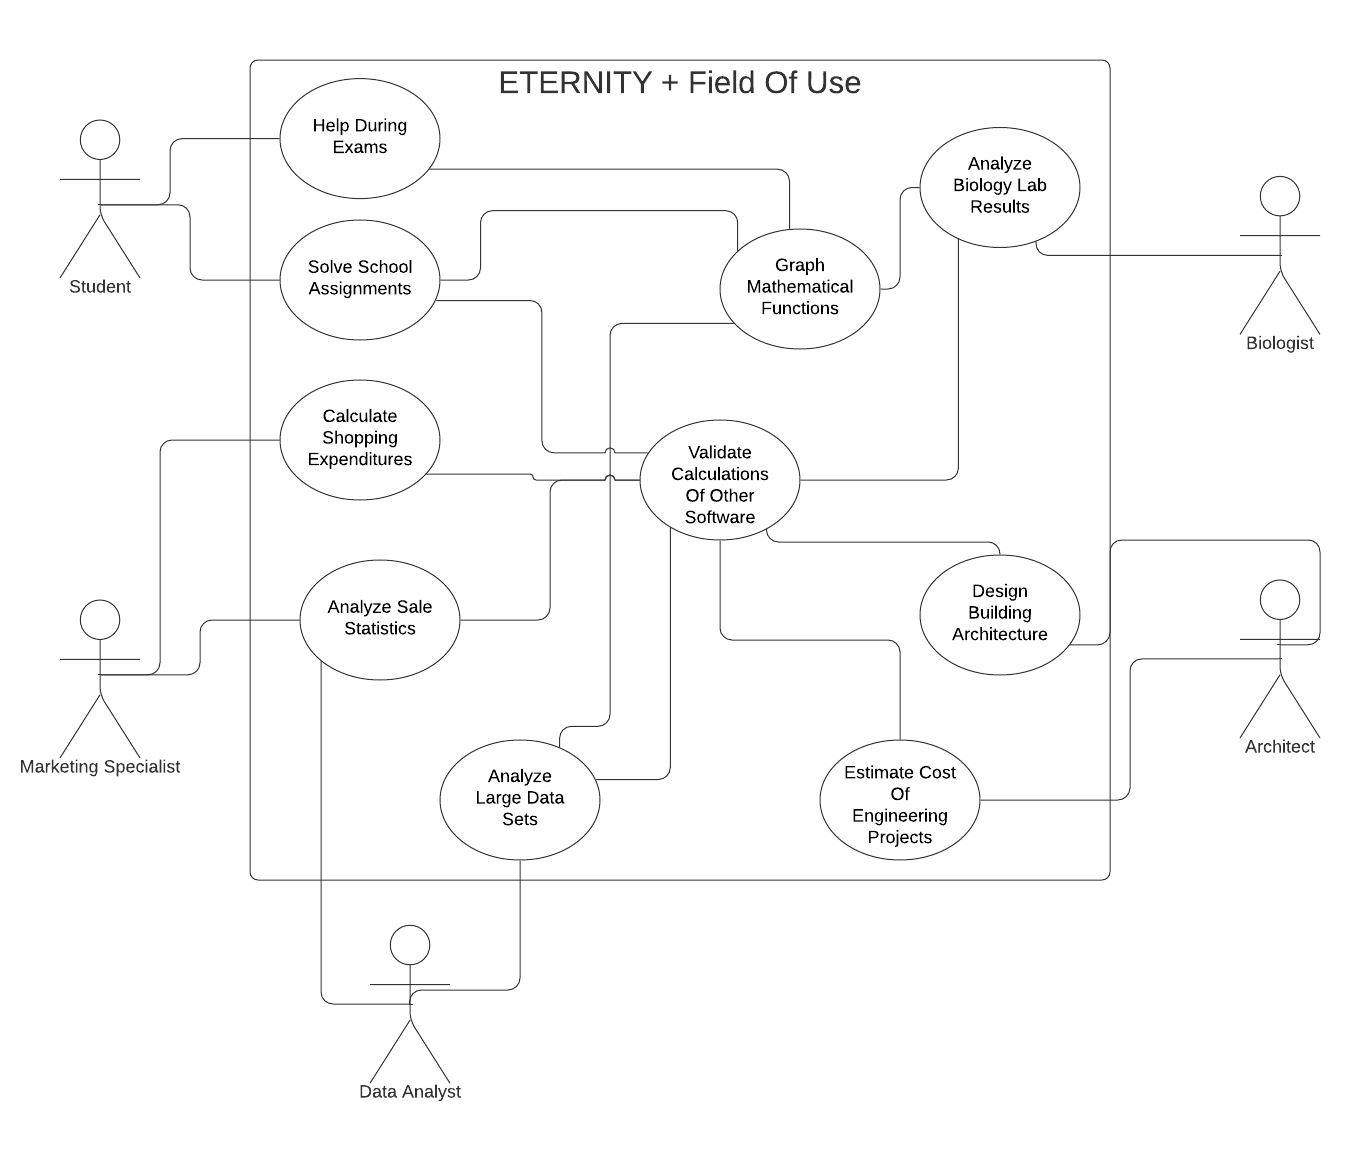
\includegraphics[scale=0.66]{images/high-level-use-case.png}
\end{center}

\subsection{Low-Level Use Cases}
\begin{center}
    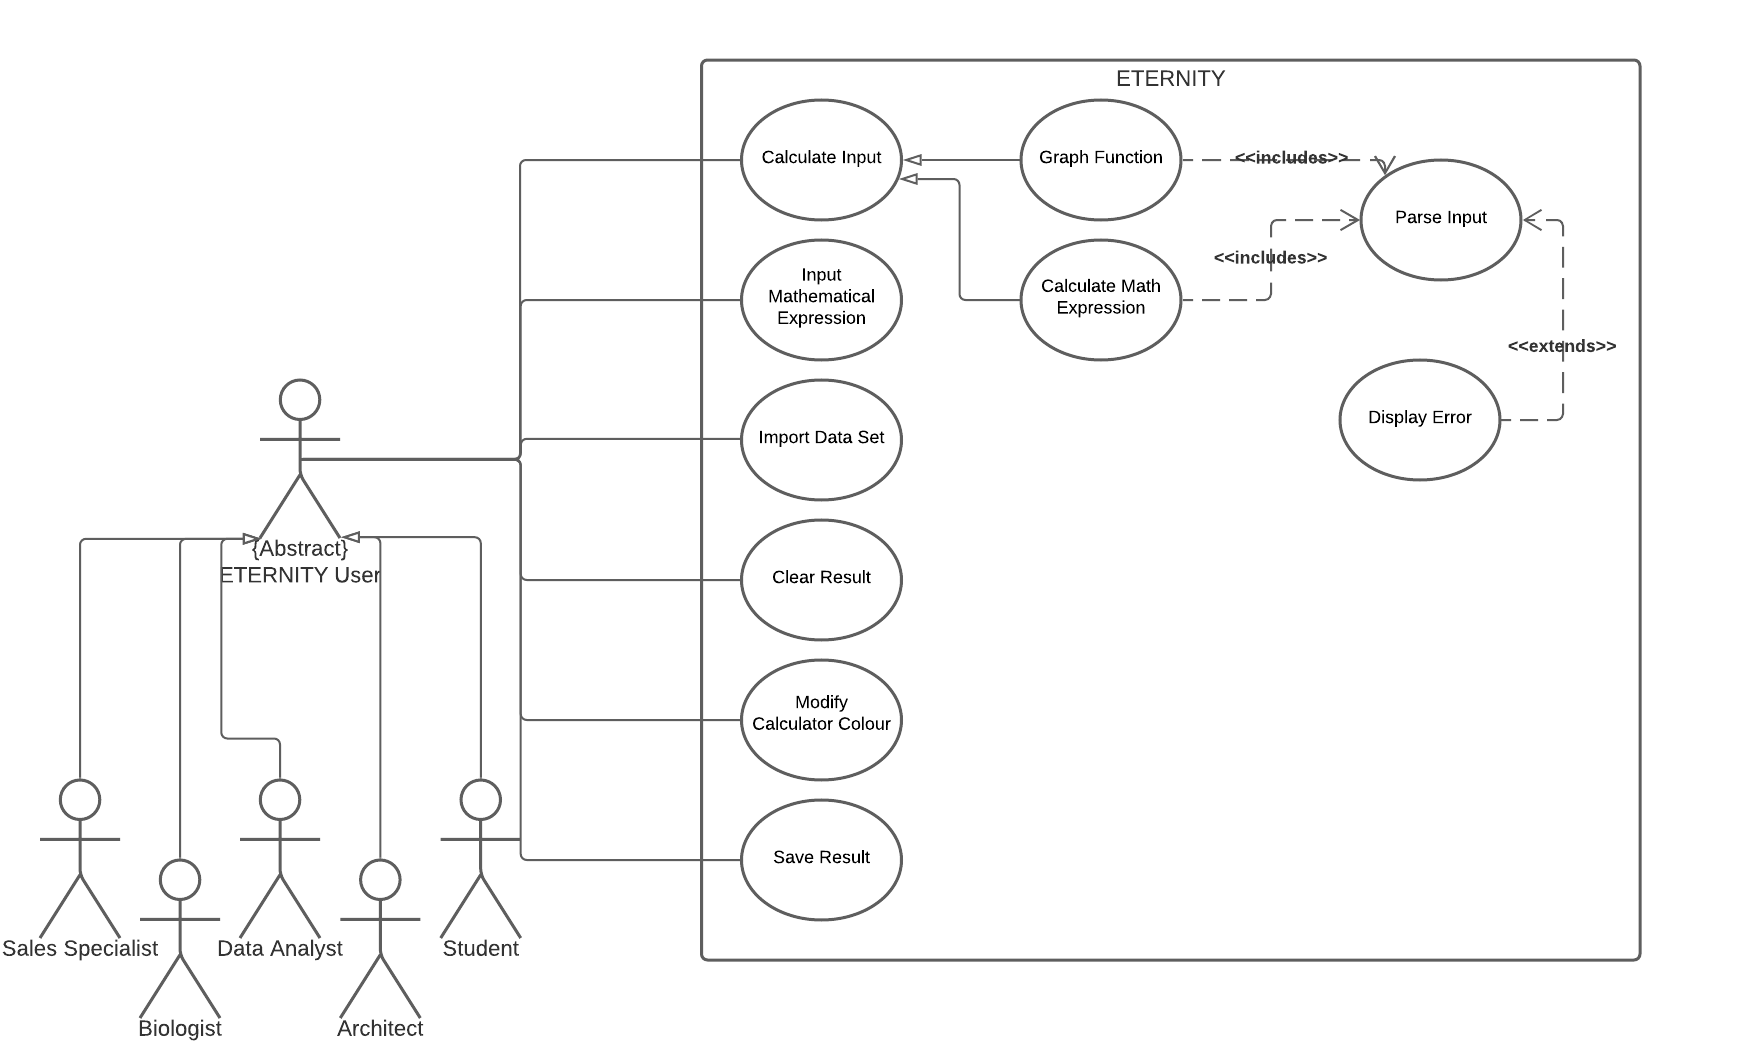
\includegraphics[scale=0.6]{images/low-level-use-case.png}
\end{center}

\bibliography{sources} 
\bibliographystyle{IEEEtran}

\begin{description}

\end{description}

\end{document}